\documentclass[1p]{elsarticle_modified}
%\bibliographystyle{elsarticle-num}

%\usepackage[colorlinks]{hyperref}
%\usepackage{abbrmath_seonhwa} %\Abb, \Ascr, \Acal ,\Abf, \Afrak
\usepackage{amsfonts}
\usepackage{amssymb}
\usepackage{amsmath}
\usepackage{amsthm}
\usepackage{scalefnt}
\usepackage{amsbsy}
\usepackage{kotex}
\usepackage{caption}
\usepackage{subfig}
\usepackage{color}
\usepackage{graphicx}
\usepackage{xcolor} %% white, black, red, green, blue, cyan, magenta, yellow
\usepackage{float}
\usepackage{setspace}
\usepackage{hyperref}

\usepackage{tikz}
\usetikzlibrary{arrows}

\usepackage{multirow}
\usepackage{array} % fixed length table
\usepackage{hhline}

%%%%%%%%%%%%%%%%%%%%%
\makeatletter
\renewcommand*\env@matrix[1][\arraystretch]{%
	\edef\arraystretch{#1}%
	\hskip -\arraycolsep
	\let\@ifnextchar\new@ifnextchar
	\array{*\c@MaxMatrixCols c}}
\makeatother %https://tex.stackexchange.com/questions/14071/how-can-i-increase-the-line-spacing-in-a-matrix
%%%%%%%%%%%%%%%

\usepackage[normalem]{ulem}

\newcommand{\msout}[1]{\ifmmode\text{\sout{\ensuremath{#1}}}\else\sout{#1}\fi}
%SOURCE: \msout is \stkout macro in https://tex.stackexchange.com/questions/20609/strikeout-in-math-mode

\newcommand{\cancel}[1]{
	\ifmmode
	{\color{red}\msout{#1}}
	\else
	{\color{red}\sout{#1}}
	\fi
}

\newcommand{\add}[1]{
	{\color{blue}\uwave{#1}}
}

\newcommand{\replace}[2]{
	\ifmmode
	{\color{red}\msout{#1}}{\color{blue}\uwave{#2}}
	\else
	{\color{red}\sout{#1}}{\color{blue}\uwave{#2}}
	\fi
}

\newcommand{\Sol}{\mathcal{S}} %segment
\newcommand{\D}{D} %diagram
\newcommand{\A}{\mathcal{A}} %arc


%%%%%%%%%%%%%%%%%%%%%%%%%%%%%5 test

\def\sl{\operatorname{\textup{SL}}(2,\Cbb)}
\def\psl{\operatorname{\textup{PSL}}(2,\Cbb)}
\def\quan{\mkern 1mu \triangleright \mkern 1mu}

\theoremstyle{definition}
\newtheorem{thm}{Theorem}[section]
\newtheorem{prop}[thm]{Proposition}
\newtheorem{lem}[thm]{Lemma}
\newtheorem{ques}[thm]{Question}
\newtheorem{cor}[thm]{Corollary}
\newtheorem{defn}[thm]{Definition}
\newtheorem{exam}[thm]{Example}
\newtheorem{rmk}[thm]{Remark}
\newtheorem{alg}[thm]{Algorithm}

\newcommand{\I}{\sqrt{-1}}
\begin{document}

%\begin{frontmatter}
%
%\title{Boundary parabolic representations of knots up to 8 crossings}
%
%%% Group authors per affiliation:
%\author{Yunhi Cho} 
%\address{Department of Mathematics, University of Seoul, Seoul, Korea}
%\ead{yhcho@uos.ac.kr}
%
%
%\author{Seonhwa Kim} %\fnref{s_kim}}
%\address{Center for Geometry and Physics, Institute for Basic Science, Pohang, 37673, Korea}
%\ead{ryeona17@ibs.re.kr}
%
%\author{Hyuk Kim}
%\address{Department of Mathematical Sciences, Seoul National University, Seoul 08826, Korea}
%\ead{hyukkim@snu.ac.kr}
%
%\author{Seokbeom Yoon}
%\address{Department of Mathematical Sciences, Seoul National University, Seoul, 08826,  Korea}
%\ead{sbyoon15@snu.ac.kr}
%
%\begin{abstract}
%We find all boundary parabolic representation of knots up to 8 crossings.
%
%\end{abstract}
%\begin{keyword}
%    \MSC[2010] 57M25 
%\end{keyword}
%
%\end{frontmatter}

%\linenumbers
%\tableofcontents
%
\newcommand\colored[1]{\textcolor{white}{\rule[-0.35ex]{0.8em}{1.4ex}}\kern-0.8em\color{red} #1}%
%\newcommand\colored[1]{\textcolor{white}{ #1}\kern-2.17ex	\textcolor{white}{ #1}\kern-1.81ex	\textcolor{white}{ #1}\kern-2.15ex\color{red}#1	}

{\Large $\underline{11a_{228}~(K11a_{228})}$}

\setlength{\tabcolsep}{10pt}
\renewcommand{\arraystretch}{1.6}
\vspace{1cm}\begin{tabular}{m{100pt}>{\centering\arraybackslash}m{274pt}}
\multirow{5}{120pt}{
	\centering
	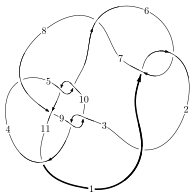
\includegraphics[width=112pt]{../../../GIT/diagram.site/Diagrams/png/477_11a_228.png}\\
\ \ \ A knot diagram\footnotemark}&
\allowdisplaybreaks
\textbf{Linearized knot diagam} \\
\cline{2-2}
 &
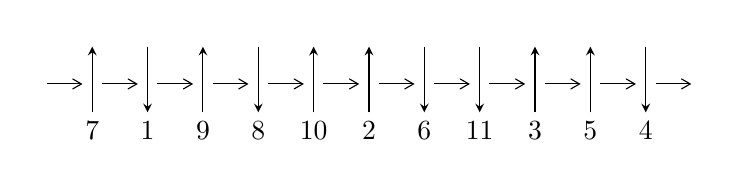
\begin{tikzpicture}[x=20pt, y=17pt]
	% nodes
	\node (C0) at (0, 0) {};
	\node (C1) at (1, 0) {};
	\node (C1U) at (1, +1) {};
	\node (C1D) at (1, -1) {7};

	\node (C2) at (2, 0) {};
	\node (C2U) at (2, +1) {};
	\node (C2D) at (2, -1) {1};

	\node (C3) at (3, 0) {};
	\node (C3U) at (3, +1) {};
	\node (C3D) at (3, -1) {9};

	\node (C4) at (4, 0) {};
	\node (C4U) at (4, +1) {};
	\node (C4D) at (4, -1) {8};

	\node (C5) at (5, 0) {};
	\node (C5U) at (5, +1) {};
	\node (C5D) at (5, -1) {10};

	\node (C6) at (6, 0) {};
	\node (C6U) at (6, +1) {};
	\node (C6D) at (6, -1) {2};

	\node (C7) at (7, 0) {};
	\node (C7U) at (7, +1) {};
	\node (C7D) at (7, -1) {6};

	\node (C8) at (8, 0) {};
	\node (C8U) at (8, +1) {};
	\node (C8D) at (8, -1) {11};

	\node (C9) at (9, 0) {};
	\node (C9U) at (9, +1) {};
	\node (C9D) at (9, -1) {3};

	\node (C10) at (10, 0) {};
	\node (C10U) at (10, +1) {};
	\node (C10D) at (10, -1) {5};

	\node (C11) at (11, 0) {};
	\node (C11U) at (11, +1) {};
	\node (C11D) at (11, -1) {4};
	\node (C12) at (12, 0) {};

	% arrows
	\draw[->,>={angle 60}]
	(C0) edge (C1) (C1) edge (C2) (C2) edge (C3) (C3) edge (C4) (C4) edge (C5) (C5) edge (C6) (C6) edge (C7) (C7) edge (C8) (C8) edge (C9) (C9) edge (C10) (C10) edge (C11) (C11) edge (C12) ;	\draw[->,>=stealth]
	(C1D) edge (C1U) (C2U) edge (C2D) (C3D) edge (C3U) (C4U) edge (C4D) (C5D) edge (C5U) (C6D) edge (C6U) (C7U) edge (C7D) (C8U) edge (C8D) (C9D) edge (C9U) (C10D) edge (C10U) (C11U) edge (C11D) ;
	\end{tikzpicture} \\
\hhline{~~} \\& 
\textbf{Solving Sequence} \\ \cline{2-2} 
 &
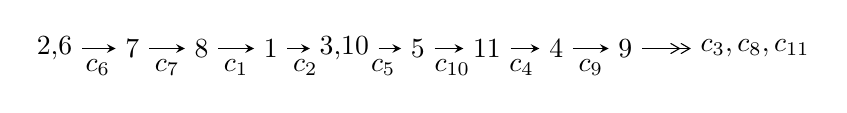
\begin{tikzpicture}[x=25pt, y=7pt]
	% node
	\node (A0) at (-1/8, 0) {2,6};
	\node (A1) at (1, 0) {7};
	\node (A2) at (2, 0) {8};
	\node (A3) at (3, 0) {1};
	\node (A4) at (65/16, 0) {3,10};
	\node (A5) at (41/8, 0) {5};
	\node (A6) at (49/8, 0) {11};
	\node (A7) at (57/8, 0) {4};
	\node (A8) at (65/8, 0) {9};
	\node (C1) at (1/2, -1) {$c_{6}$};
	\node (C2) at (3/2, -1) {$c_{7}$};
	\node (C3) at (5/2, -1) {$c_{1}$};
	\node (C4) at (7/2, -1) {$c_{2}$};
	\node (C5) at (37/8, -1) {$c_{5}$};
	\node (C6) at (45/8, -1) {$c_{10}$};
	\node (C7) at (53/8, -1) {$c_{4}$};
	\node (C8) at (61/8, -1) {$c_{9}$};
	\node (A9) at (10, 0) {$c_{3},c_{8},c_{11}$};

	% edge
	\draw[->,>=stealth]	
	(A0) edge (A1) (A1) edge (A2) (A2) edge (A3) (A3) edge (A4) (A4) edge (A5) (A5) edge (A6) (A6) edge (A7) (A7) edge (A8) ;
	\draw[->>,>={angle 60}]	
	(A8) edge (A9);
\end{tikzpicture} \\ 

\end{tabular} \\

\footnotetext{
The image of knot diagram is generated by the software ``\textbf{Draw programme}" developed by Andrew Bartholomew(\url{http://www.layer8.co.uk/maths/draw/index.htm\#Running-draw}), where we modified some parts for our purpose(\url{https://github.com/CATsTAILs/LinksPainter}).
}\phantom \\ \newline 
\centering \textbf{Ideals for irreducible components\footnotemark of $X_{\text{par}}$} 
 
\begin{align*}
I^u_{1}&=\langle 
-15 u^{25}-53 u^{24}+\cdots+4 b+140,\;-29 u^{25}-269 u^{24}+\cdots+8 a-580,\;u^{26}+7 u^{25}+\cdots+12 u+8\rangle \\
I^u_{2}&=\langle 
8.51292\times10^{18} a^{5} u^{8}-1.75570\times10^{19} a^{4} u^{8}+\cdots+2.60029\times10^{20} a-4.53756\times10^{20},\\
\phantom{I^u_{2}}&\phantom{= \langle  }-2 u^8 a^4-7 u^8 a^3+\cdots-9 a+6,\;u^9- u^8+2 u^7- u^6+3 u^5- u^4+2 u^3+u+1\rangle \\
I^u_{3}&=\langle 
u^{11}+2 u^9+4 u^7- u^6+5 u^5- u^4+3 u^3- u^2+b+2 u,\\
\phantom{I^u_{3}}&\phantom{= \langle  }- u^{13}- u^{12}-3 u^{11}-2 u^{10}-7 u^9-3 u^8-9 u^7-2 u^6-9 u^5+u^4-6 u^3+u^2+a-2 u+2,\\
\phantom{I^u_{3}}&\phantom{= \langle  }u^{14}+3 u^{12}+7 u^{10}- u^9+11 u^8-2 u^7+12 u^6-3 u^5+10 u^4-2 u^3+5 u^2- u+1\rangle \\
\\
\end{align*}
\raggedright * 3 irreducible components of $\dim_{\mathbb{C}}=0$, with total 94 representations.\\
\footnotetext{All coefficients of polynomials are rational numbers. But the coefficients are sometimes approximated in decimal forms when there is not enough margin.}
\newpage
\renewcommand{\arraystretch}{1}
\centering \section*{I. $I^u_{1}= \langle -15 u^{25}-53 u^{24}+\cdots+4 b+140,\;-29 u^{25}-269 u^{24}+\cdots+8 a-580,\;u^{26}+7 u^{25}+\cdots+12 u+8 \rangle$}
\flushleft \textbf{(i) Arc colorings}\\
\begin{tabular}{m{7pt} m{180pt} m{7pt} m{180pt} }
\flushright $a_{2}=$&$\begin{pmatrix}0\\u\end{pmatrix}$ \\
\flushright $a_{6}=$&$\begin{pmatrix}1\\0\end{pmatrix}$ \\
\flushright $a_{7}=$&$\begin{pmatrix}1\\- u^2\end{pmatrix}$ \\
\flushright $a_{8}=$&$\begin{pmatrix}u^2+1\\- u^2\end{pmatrix}$ \\
\flushright $a_{1}=$&$\begin{pmatrix}- u\\u^3+u\end{pmatrix}$ \\
\flushright $a_{3}=$&$\begin{pmatrix}- u^3\\u^5+u^3+u\end{pmatrix}$ \\
\flushright $a_{10}=$&$\begin{pmatrix}3.62500 u^{25}+33.6250 u^{24}+\cdots+49.2500 u+72.5000\\\frac{15}{4} u^{25}+\frac{53}{4} u^{24}+\cdots+5 u-35\end{pmatrix}$ \\
\flushright $a_{5}=$&$\begin{pmatrix}\frac{63}{8} u^{25}+\frac{371}{8} u^{24}+\cdots+\frac{197}{4} u+24\\-\frac{25}{4} u^{25}-\frac{161}{4} u^{24}+\cdots-\frac{97}{2} u-37\end{pmatrix}$ \\
\flushright $a_{11}=$&$\begin{pmatrix}\frac{41}{8} u^{25}+\frac{335}{8} u^{24}+\cdots+\frac{119}{2} u+85\\6 u^{25}+\frac{53}{2} u^{24}+\cdots+\frac{45}{2} u-41\end{pmatrix}$ \\
\flushright $a_{4}=$&$\begin{pmatrix}\frac{9}{8} u^{25}+\frac{61}{8} u^{24}+\cdots+\frac{59}{4} u+1\\-\frac{1}{4} u^{25}-\frac{13}{4} u^{24}+\cdots-\frac{25}{2} u-9\end{pmatrix}$ \\
\flushright $a_{9}=$&$\begin{pmatrix}-3.37500 u^{25}-27.3750 u^{24}+\cdots-38.7500 u-55.5000\\-\frac{21}{4} u^{25}-\frac{103}{4} u^{24}+\cdots-27 u+27\end{pmatrix}$\\ \flushright $a_{9}=$&$\begin{pmatrix}-3.37500 u^{25}-27.3750 u^{24}+\cdots-38.7500 u-55.5000\\-\frac{21}{4} u^{25}-\frac{103}{4} u^{24}+\cdots-27 u+27\end{pmatrix}$\\&\end{tabular}
\flushleft \textbf{(ii) Obstruction class $= -1$}\\~\\
\flushleft \textbf{(iii) Cusp Shapes $= -12 u^{25}-78 u^{24}-301 u^{23}-809 u^{22}-1723 u^{21}-2988 u^{20}-4360 u^{19}-5258 u^{18}-5163 u^{17}-3679 u^{16}-1188 u^{15}+1603 u^{14}+3423 u^{13}+3726 u^{12}+2364 u^{11}+364 u^{10}-1475 u^9-2219 u^8-2061 u^7-1330 u^6-696 u^5-201 u^4-18 u^3-43 u^2-116 u-58$}\\~\\
\newpage\renewcommand{\arraystretch}{1}
\flushleft \textbf{(iv) u-Polynomials at the component}\newline \\
\begin{tabular}{m{50pt}|m{274pt}}
Crossings & \hspace{64pt}u-Polynomials at each crossing \\
\hline $$\begin{aligned}c_{1},c_{6}\end{aligned}$$&$\begin{aligned}
&u^{26}+7 u^{25}+\cdots+12 u+8
\end{aligned}$\\
\hline $$\begin{aligned}c_{2},c_{7}\end{aligned}$$&$\begin{aligned}
&u^{26}+9 u^{25}+\cdots+48 u+64
\end{aligned}$\\
\hline $$\begin{aligned}c_{3},c_{5},c_{9}\\c_{10}\end{aligned}$$&$\begin{aligned}
&u^{26}+8 u^{24}+\cdots+2 u+1
\end{aligned}$\\
\hline $$\begin{aligned}c_{4},c_{11}\end{aligned}$$&$\begin{aligned}
&u^{26}- u^{25}+\cdots-3 u+1
\end{aligned}$\\
\hline $$\begin{aligned}c_{8}\end{aligned}$$&$\begin{aligned}
&u^{26}-21 u^{25}+\cdots-6912 u+512
\end{aligned}$\\
\hline
\end{tabular}\\~\\
\newpage\renewcommand{\arraystretch}{1}
\flushleft \textbf{(v) Riley Polynomials at the component}\newline \\
\begin{tabular}{m{50pt}|m{274pt}}
Crossings & \hspace{64pt}Riley Polynomials at each crossing \\
\hline $$\begin{aligned}c_{1},c_{6}\end{aligned}$$&$\begin{aligned}
&y^{26}+9 y^{25}+\cdots+48 y+64
\end{aligned}$\\
\hline $$\begin{aligned}c_{2},c_{7}\end{aligned}$$&$\begin{aligned}
&y^{26}+17 y^{25}+\cdots+60160 y+4096
\end{aligned}$\\
\hline $$\begin{aligned}c_{3},c_{5},c_{9}\\c_{10}\end{aligned}$$&$\begin{aligned}
&y^{26}+16 y^{25}+\cdots-2 y+1
\end{aligned}$\\
\hline $$\begin{aligned}c_{4},c_{11}\end{aligned}$$&$\begin{aligned}
&y^{26}+9 y^{25}+\cdots+19 y+1
\end{aligned}$\\
\hline $$\begin{aligned}c_{8}\end{aligned}$$&$\begin{aligned}
&y^{26}-5 y^{25}+\cdots+196608 y+262144
\end{aligned}$\\
\hline
\end{tabular}\\~\\
\newpage\flushleft \textbf{(vi) Complex Volumes and Cusp Shapes}
$$\begin{array}{c|c|c}  
\text{Solutions to }I^u_{1}& \I (\text{vol} + \sqrt{-1}CS) & \text{Cusp shape}\\
 \hline 
\begin{aligned}
u &= -0.837651 + 0.572406 I \\
a &= \phantom{-}0.835566 + 0.354168 I \\
b &= -0.531846 - 0.873998 I\end{aligned}
 & \phantom{-}1.84430 + 3.12249 I & \phantom{-}4.20356 - 5.13534 I \\ \hline\begin{aligned}
u &= -0.837651 - 0.572406 I \\
a &= \phantom{-}0.835566 - 0.354168 I \\
b &= -0.531846 + 0.873998 I\end{aligned}
 & \phantom{-}1.84430 - 3.12249 I & \phantom{-}4.20356 + 5.13534 I \\ \hline\begin{aligned}
u &= \phantom{-}0.881347 + 0.183622 I \\
a &= -0.573452 - 0.801837 I \\
b &= \phantom{-}0.396890 + 1.190540 I\end{aligned}
 & -3.96770 + 6.65430 I & -0.65787 - 6.33935 I \\ \hline\begin{aligned}
u &= \phantom{-}0.881347 - 0.183622 I \\
a &= -0.573452 + 0.801837 I \\
b &= \phantom{-}0.396890 - 1.190540 I\end{aligned}
 & -3.96770 - 6.65430 I & -0.65787 + 6.33935 I \\ \hline\begin{aligned}
u &= \phantom{-}0.297455 + 0.831482 I \\
a &= \phantom{-}0.191314 + 0.562862 I \\
b &= \phantom{-}0.504051 - 0.077620 I\end{aligned}
 & -0.64079 + 1.97179 I & \phantom{-}1.39932 - 4.26013 I \\ \hline\begin{aligned}
u &= \phantom{-}0.297455 - 0.831482 I \\
a &= \phantom{-}0.191314 - 0.562862 I \\
b &= \phantom{-}0.504051 + 0.077620 I\end{aligned}
 & -0.64079 - 1.97179 I & \phantom{-}1.39932 + 4.26013 I \\ \hline\begin{aligned}
u &= -0.899623 + 0.665417 I \\
a &= -0.786099 - 0.972145 I \\
b &= \phantom{-}0.63545 + 1.32692 I\end{aligned}
 & -1.14356 + 10.71300 I & \phantom{-}0.33526 - 5.40937 I \\ \hline\begin{aligned}
u &= -0.899623 - 0.665417 I \\
a &= -0.786099 + 0.972145 I \\
b &= \phantom{-}0.63545 - 1.32692 I\end{aligned}
 & -1.14356 - 10.71300 I & \phantom{-}0.33526 + 5.40937 I \\ \hline\begin{aligned}
u &= -0.800652 + 0.839278 I \\
a &= \phantom{-}1.244260 + 0.159972 I \\
b &= -0.866677 + 0.161865 I\end{aligned}
 & \phantom{-}5.83701 - 0.85262 I & \phantom{-}7.15266 + 0.82662 I \\ \hline\begin{aligned}
u &= -0.800652 - 0.839278 I \\
a &= \phantom{-}1.244260 - 0.159972 I \\
b &= -0.866677 - 0.161865 I\end{aligned}
 & \phantom{-}5.83701 + 0.85262 I & \phantom{-}7.15266 - 0.82662 I\\
 \hline 
 \end{array}$$\newpage$$\begin{array}{c|c|c}  
\text{Solutions to }I^u_{1}& \I (\text{vol} + \sqrt{-1}CS) & \text{Cusp shape}\\
 \hline 
\begin{aligned}
u &= \phantom{-}0.201343 + 1.171450 I \\
a &= \phantom{-}0.634705 - 1.046330 I \\
b &= -0.44754 - 1.35708 I\end{aligned}
 & -8.67640 + 10.06980 I & -5.88892 - 7.31379 I \\ \hline\begin{aligned}
u &= \phantom{-}0.201343 - 1.171450 I \\
a &= \phantom{-}0.634705 + 1.046330 I \\
b &= -0.44754 + 1.35708 I\end{aligned}
 & -8.67640 - 10.06980 I & -5.88892 + 7.31379 I \\ \hline\begin{aligned}
u &= -0.093471 + 1.199340 I \\
a &= -0.073401 + 0.980820 I \\
b &= \phantom{-}0.239568 + 0.837324 I\end{aligned}
 & -4.09225 + 1.31670 I & \phantom{-}5.84188 - 2.64117 I \\ \hline\begin{aligned}
u &= -0.093471 - 1.199340 I \\
a &= -0.073401 - 0.980820 I \\
b &= \phantom{-}0.239568 - 0.837324 I\end{aligned}
 & -4.09225 - 1.31670 I & \phantom{-}5.84188 + 2.64117 I \\ \hline\begin{aligned}
u &= -0.781122 + 0.922042 I \\
a &= -0.938819 - 0.875292 I \\
b &= \phantom{-}0.846844 + 0.063440 I\end{aligned}
 & \phantom{-}5.58632 - 5.07870 I & \phantom{-}6.80297 + 4.99584 I \\ \hline\begin{aligned}
u &= -0.781122 - 0.922042 I \\
a &= -0.938819 + 0.875292 I \\
b &= \phantom{-}0.846844 - 0.063440 I\end{aligned}
 & \phantom{-}5.58632 + 5.07870 I & \phantom{-}6.80297 - 4.99584 I \\ \hline\begin{aligned}
u &= \phantom{-}0.439531 + 1.186270 I \\
a &= -0.784277 + 0.187768 I \\
b &= -0.232529 + 1.203110 I\end{aligned}
 & -7.23748 - 1.85191 I & -5.27925 + 3.38649 I \\ \hline\begin{aligned}
u &= \phantom{-}0.439531 - 1.186270 I \\
a &= -0.784277 - 0.187768 I \\
b &= -0.232529 - 1.203110 I\end{aligned}
 & -7.23748 + 1.85191 I & -5.27925 - 3.38649 I \\ \hline\begin{aligned}
u &= -0.698499 + 1.080440 I \\
a &= -1.60109 - 0.59030 I \\
b &= \phantom{-}0.513688 - 0.994028 I\end{aligned}
 & \phantom{-}0.31911 - 8.88087 I & \phantom{-}0.68625 + 10.27634 I \\ \hline\begin{aligned}
u &= -0.698499 - 1.080440 I \\
a &= -1.60109 + 0.59030 I \\
b &= \phantom{-}0.513688 + 0.994028 I\end{aligned}
 & \phantom{-}0.31911 + 8.88087 I & \phantom{-}0.68625 - 10.27634 I\\
 \hline 
 \end{array}$$\newpage$$\begin{array}{c|c|c}  
\text{Solutions to }I^u_{1}& \I (\text{vol} + \sqrt{-1}CS) & \text{Cusp shape}\\
 \hline 
\begin{aligned}
u &= -0.749005 + 1.057380 I \\
a &= \phantom{-}2.09827 + 0.24225 I \\
b &= -0.65034 + 1.38923 I\end{aligned}
 & -2.3566 - 16.8090 I & -1.24843 + 9.63879 I \\ \hline\begin{aligned}
u &= -0.749005 - 1.057380 I \\
a &= \phantom{-}2.09827 - 0.24225 I \\
b &= -0.65034 - 1.38923 I\end{aligned}
 & -2.3566 + 16.8090 I & -1.24843 - 9.63879 I \\ \hline\begin{aligned}
u &= -0.932872 + 0.931207 I \\
a &= -0.472447 + 0.573546 I \\
b &= \phantom{-}0.053787 - 0.847257 I\end{aligned}
 & \phantom{-}3.75978 - 3.40349 I & -4.66696 + 3.91131 I \\ \hline\begin{aligned}
u &= -0.932872 - 0.931207 I \\
a &= -0.472447 - 0.573546 I \\
b &= \phantom{-}0.053787 + 0.847257 I\end{aligned}
 & \phantom{-}3.75978 + 3.40349 I & -4.66696 - 3.91131 I \\ \hline\begin{aligned}
u &= \phantom{-}0.473220 + 0.303991 I \\
a &= \phantom{-}0.975471 + 0.017379 I \\
b &= -0.461342 - 0.420051 I\end{aligned}
 & \phantom{-}0.898620 + 0.817519 I & \phantom{-}6.81953 - 4.33053 I \\ \hline\begin{aligned}
u &= \phantom{-}0.473220 - 0.303991 I \\
a &= \phantom{-}0.975471 - 0.017379 I \\
b &= -0.461342 + 0.420051 I\end{aligned}
 & \phantom{-}0.898620 - 0.817519 I & \phantom{-}6.81953 + 4.33053 I\\
 \hline 
 \end{array}$$\newpage\newpage\renewcommand{\arraystretch}{1}
\centering \section*{II. $I^u_{2}= \langle 8.51\times10^{18} a^{5} u^{8}-1.76\times10^{19} a^{4} u^{8}+\cdots+2.60\times10^{20} a-4.54\times10^{20},\;-2 u^8 a^4-7 u^8 a^3+\cdots-9 a+6,\;u^9- u^8+2 u^7- u^6+3 u^5- u^4+2 u^3+u+1 \rangle$}
\flushleft \textbf{(i) Arc colorings}\\
\begin{tabular}{m{7pt} m{180pt} m{7pt} m{180pt} }
\flushright $a_{2}=$&$\begin{pmatrix}0\\u\end{pmatrix}$ \\
\flushright $a_{6}=$&$\begin{pmatrix}1\\0\end{pmatrix}$ \\
\flushright $a_{7}=$&$\begin{pmatrix}1\\- u^2\end{pmatrix}$ \\
\flushright $a_{8}=$&$\begin{pmatrix}u^2+1\\- u^2\end{pmatrix}$ \\
\flushright $a_{1}=$&$\begin{pmatrix}- u\\u^3+u\end{pmatrix}$ \\
\flushright $a_{3}=$&$\begin{pmatrix}- u^3\\u^5+u^3+u\end{pmatrix}$ \\
\flushright $a_{10}=$&$\begin{pmatrix}a\\-0.0501691 a^{5} u^{8}+0.103468 a^{4} u^{8}+\cdots-1.53242 a+2.67411\end{pmatrix}$ \\
\flushright $a_{5}=$&$\begin{pmatrix}0.0104893 a^{5} u^{8}+0.300793 a^{4} u^{8}+\cdots-1.19290 a+4.00869\\0.0757787 a^{5} u^{8}+0.141035 a^{4} u^{8}+\cdots+2.09572 a-3.59647\end{pmatrix}$ \\
\flushright $a_{11}=$&$\begin{pmatrix}-0.0191376 a^{5} u^{8}+0.302267 a^{4} u^{8}+\cdots+0.192227 a-0.0413771\\0.0842588 a^{5} u^{8}-0.190487 a^{4} u^{8}+\cdots-1.41715 a+1.39892\end{pmatrix}$ \\
\flushright $a_{4}=$&$\begin{pmatrix}-0.0505824 a^{5} u^{8}-0.230088 a^{4} u^{8}+\cdots+0.271748 a+0.149238\\0.0624037 a^{5} u^{8}+0.372711 a^{4} u^{8}+\cdots+1.33349 a-2.66894\end{pmatrix}$ \\
\flushright $a_{9}=$&$\begin{pmatrix}-0.117790 a^{5} u^{8}+0.236604 a^{4} u^{8}+\cdots+0.487696 a-0.491448\\0.144583 a^{5} u^{8}+0.0202877 a^{4} u^{8}+\cdots-1.10453 a+2.79806\end{pmatrix}$\\ \flushright $a_{9}=$&$\begin{pmatrix}-0.117790 a^{5} u^{8}+0.236604 a^{4} u^{8}+\cdots+0.487696 a-0.491448\\0.144583 a^{5} u^{8}+0.0202877 a^{4} u^{8}+\cdots-1.10453 a+2.79806\end{pmatrix}$\\&\end{tabular}
\flushleft \textbf{(ii) Obstruction class $= -1$}\\~\\
\flushleft \textbf{(iii) Cusp Shapes $= -\frac{1848468244326230304}{24240666886441401379} u^8 a^5+\frac{7769797230450955500}{24240666886441401379} u^8 a^4+\cdots-\frac{86732149638444774432}{24240666886441401379} a+\frac{198450488198204972058}{24240666886441401379}$}\\~\\
\newpage\renewcommand{\arraystretch}{1}
\flushleft \textbf{(iv) u-Polynomials at the component}\newline \\
\begin{tabular}{m{50pt}|m{274pt}}
Crossings & \hspace{64pt}u-Polynomials at each crossing \\
\hline $$\begin{aligned}c_{1},c_{6}\end{aligned}$$&$\begin{aligned}
&(u^9- u^8+2 u^7- u^6+3 u^5- u^4+2 u^3+u+1)^6
\end{aligned}$\\
\hline $$\begin{aligned}c_{2},c_{7}\end{aligned}$$&$\begin{aligned}
&(u^9+3 u^8+8 u^7+13 u^6+17 u^5+17 u^4+12 u^3+6 u^2+u-1)^6
\end{aligned}$\\
\hline $$\begin{aligned}c_{3},c_{5},c_{9}\\c_{10}\end{aligned}$$&$\begin{aligned}
&u^{54}- u^{53}+\cdots+2026 u+167
\end{aligned}$\\
\hline $$\begin{aligned}c_{4},c_{11}\end{aligned}$$&$\begin{aligned}
&u^{54}-3 u^{53}+\cdots-88 u+7
\end{aligned}$\\
\hline $$\begin{aligned}c_{8}\end{aligned}$$&$\begin{aligned}
&(u^3+u^2-1)^{18}
\end{aligned}$\\
\hline
\end{tabular}\\~\\
\newpage\renewcommand{\arraystretch}{1}
\flushleft \textbf{(v) Riley Polynomials at the component}\newline \\
\begin{tabular}{m{50pt}|m{274pt}}
Crossings & \hspace{64pt}Riley Polynomials at each crossing \\
\hline $$\begin{aligned}c_{1},c_{6}\end{aligned}$$&$\begin{aligned}
&(y^9+3 y^8+8 y^7+13 y^6+17 y^5+17 y^4+12 y^3+6 y^2+y-1)^6
\end{aligned}$\\
\hline $$\begin{aligned}c_{2},c_{7}\end{aligned}$$&$\begin{aligned}
&(y^9+7 y^8+20 y^7+25 y^6+5 y^5-15 y^4+22 y^2+13 y-1)^6
\end{aligned}$\\
\hline $$\begin{aligned}c_{3},c_{5},c_{9}\\c_{10}\end{aligned}$$&$\begin{aligned}
&y^{54}+39 y^{53}+\cdots-756660 y+27889
\end{aligned}$\\
\hline $$\begin{aligned}c_{4},c_{11}\end{aligned}$$&$\begin{aligned}
&y^{54}-13 y^{53}+\cdots-772 y+49
\end{aligned}$\\
\hline $$\begin{aligned}c_{8}\end{aligned}$$&$\begin{aligned}
&(y^3- y^2+2 y-1)^{18}
\end{aligned}$\\
\hline
\end{tabular}\\~\\
\newpage\flushleft \textbf{(vi) Complex Volumes and Cusp Shapes}
$$\begin{array}{c|c|c}  
\text{Solutions to }I^u_{2}& \I (\text{vol} + \sqrt{-1}CS) & \text{Cusp shape}\\
 \hline 
\begin{aligned}
u &= -0.140343 + 0.966856 I \\
a &= -0.789673 + 0.879642 I \\
b &= \phantom{-}0.197045 + 0.055587 I\end{aligned}
 & -3.69411 + 0.73475 I & -5.00524 + 1.18338 I \\ \hline\begin{aligned}
u &= -0.140343 + 0.966856 I \\
a &= \phantom{-}0.80190 + 1.19171 I \\
b &= -0.51815 + 1.57690 I\end{aligned}
 & -7.83169 - 2.09337 I & -11.53450 + 4.16283 I \\ \hline\begin{aligned}
u &= -0.140343 + 0.966856 I \\
a &= \phantom{-}0.32744 + 1.40287 I \\
b &= \phantom{-}0.303816 + 1.064500 I\end{aligned}
 & -3.69411 + 0.73475 I & -5.00524 + 1.18338 I \\ \hline\begin{aligned}
u &= -0.140343 + 0.966856 I \\
a &= \phantom{-}0.158893 + 0.006810 I \\
b &= -1.104640 + 0.259039 I\end{aligned}
 & -3.69411 - 4.92150 I & -5.00524 + 7.14228 I \\ \hline\begin{aligned}
u &= -0.140343 + 0.966856 I \\
a &= -1.80300 - 1.22850 I \\
b &= \phantom{-}0.077708 - 1.286090 I\end{aligned}
 & -7.83169 - 2.09337 I & -11.53450 + 4.16283 I \\ \hline\begin{aligned}
u &= -0.140343 + 0.966856 I \\
a &= -0.45237 - 2.31709 I \\
b &= \phantom{-}0.271297 - 1.159590 I\end{aligned}
 & -3.69411 - 4.92150 I & -5.00524 + 7.14228 I \\ \hline\begin{aligned}
u &= -0.140343 - 0.966856 I \\
a &= -0.789673 - 0.879642 I \\
b &= \phantom{-}0.197045 - 0.055587 I\end{aligned}
 & -3.69411 - 0.73475 I & -5.00524 - 1.18338 I \\ \hline\begin{aligned}
u &= -0.140343 - 0.966856 I \\
a &= \phantom{-}0.80190 - 1.19171 I \\
b &= -0.51815 - 1.57690 I\end{aligned}
 & -7.83169 + 2.09337 I & -11.53450 - 4.16283 I \\ \hline\begin{aligned}
u &= -0.140343 - 0.966856 I \\
a &= \phantom{-}0.32744 - 1.40287 I \\
b &= \phantom{-}0.303816 - 1.064500 I\end{aligned}
 & -3.69411 - 0.73475 I & -5.00524 - 1.18338 I \\ \hline\begin{aligned}
u &= -0.140343 - 0.966856 I \\
a &= \phantom{-}0.158893 - 0.006810 I \\
b &= -1.104640 - 0.259039 I\end{aligned}
 & -3.69411 + 4.92150 I & -5.00524 - 7.14228 I\\
 \hline 
 \end{array}$$\newpage$$\begin{array}{c|c|c}  
\text{Solutions to }I^u_{2}& \I (\text{vol} + \sqrt{-1}CS) & \text{Cusp shape}\\
 \hline 
\begin{aligned}
u &= -0.140343 - 0.966856 I \\
a &= -1.80300 + 1.22850 I \\
b &= \phantom{-}0.077708 + 1.286090 I\end{aligned}
 & -7.83169 + 2.09337 I & -11.53450 - 4.16283 I \\ \hline\begin{aligned}
u &= -0.140343 - 0.966856 I \\
a &= -0.45237 + 2.31709 I \\
b &= \phantom{-}0.271297 + 1.159590 I\end{aligned}
 & -3.69411 + 4.92150 I & -5.00524 - 7.14228 I \\ \hline\begin{aligned}
u &= -0.628449 + 0.875112 I \\
a &= \phantom{-}0.942165 + 0.601863 I \\
b &= \phantom{-}0.02614 + 1.49190 I\end{aligned}
 & -5.43132 - 2.45442 I & -8.69159 + 2.91298 I \\ \hline\begin{aligned}
u &= -0.628449 + 0.875112 I \\
a &= -1.262370 - 0.229556 I \\
b &= \phantom{-}0.173732 + 0.700808 I\end{aligned}
 & -1.29373 - 5.28254 I & -2.16232 + 5.89242 I \\ \hline\begin{aligned}
u &= -0.628449 + 0.875112 I \\
a &= \phantom{-}1.08622 + 1.35134 I \\
b &= -0.923600 - 0.879737 I\end{aligned}
 & -1.293730 + 0.373705 I & -2.16232 - 0.06647 I \\ \hline\begin{aligned}
u &= -0.628449 + 0.875112 I \\
a &= -1.52683 + 0.97782 I \\
b &= -0.10677 - 1.91340 I\end{aligned}
 & -5.43132 - 2.45442 I & -8.69159 + 2.91298 I \\ \hline\begin{aligned}
u &= -0.628449 + 0.875112 I \\
a &= \phantom{-}2.31670 + 0.58603 I \\
b &= -0.073681 + 0.905589 I\end{aligned}
 & -1.293730 + 0.373705 I & -2.16232 - 0.06647 I \\ \hline\begin{aligned}
u &= -0.628449 + 0.875112 I \\
a &= -2.58190 - 0.51535 I \\
b &= \phantom{-}0.762688 - 1.044840 I\end{aligned}
 & -1.29373 - 5.28254 I & -2.16232 + 5.89242 I \\ \hline\begin{aligned}
u &= -0.628449 - 0.875112 I \\
a &= \phantom{-}0.942165 - 0.601863 I \\
b &= \phantom{-}0.02614 - 1.49190 I\end{aligned}
 & -5.43132 + 2.45442 I & -8.69159 - 2.91298 I \\ \hline\begin{aligned}
u &= -0.628449 - 0.875112 I \\
a &= -1.262370 + 0.229556 I \\
b &= \phantom{-}0.173732 - 0.700808 I\end{aligned}
 & -1.29373 + 5.28254 I & -2.16232 - 5.89242 I\\
 \hline 
 \end{array}$$\newpage$$\begin{array}{c|c|c}  
\text{Solutions to }I^u_{2}& \I (\text{vol} + \sqrt{-1}CS) & \text{Cusp shape}\\
 \hline 
\begin{aligned}
u &= -0.628449 - 0.875112 I \\
a &= \phantom{-}1.08622 - 1.35134 I \\
b &= -0.923600 + 0.879737 I\end{aligned}
 & -1.293730 - 0.373705 I & -2.16232 + 0.06647 I \\ \hline\begin{aligned}
u &= -0.628449 - 0.875112 I \\
a &= -1.52683 - 0.97782 I \\
b &= -0.10677 + 1.91340 I\end{aligned}
 & -5.43132 + 2.45442 I & -8.69159 - 2.91298 I \\ \hline\begin{aligned}
u &= -0.628449 - 0.875112 I \\
a &= \phantom{-}2.31670 - 0.58603 I \\
b &= -0.073681 - 0.905589 I\end{aligned}
 & -1.293730 - 0.373705 I & -2.16232 + 0.06647 I \\ \hline\begin{aligned}
u &= -0.628449 - 0.875112 I \\
a &= -2.58190 + 0.51535 I \\
b &= \phantom{-}0.762688 + 1.044840 I\end{aligned}
 & -1.29373 + 5.28254 I & -2.16232 - 5.89242 I \\ \hline\begin{aligned}
u &= \phantom{-}0.796005 + 0.733148 I \\
a &= \phantom{-}0.713362 - 0.505363 I \\
b &= -0.502274 + 1.249400 I\end{aligned}
 & \phantom{-}2.46068 - 4.16429 I & \phantom{-}2.79385 + 3.68120 I \\ \hline\begin{aligned}
u &= \phantom{-}0.796005 + 0.733148 I \\
a &= \phantom{-}1.238440 + 0.048506 I \\
b &= -0.648327 - 0.667502 I\end{aligned}
 & \phantom{-}2.46068 + 1.49195 I & \phantom{-}2.79385 - 2.27770 I \\ \hline\begin{aligned}
u &= \phantom{-}0.796005 + 0.733148 I \\
a &= \phantom{-}0.765974 - 1.136570 I \\
b &= -0.118171 + 0.986357 I\end{aligned}
 & -1.67691 - 1.33617 I & -3.73542 + 0.70175 I \\ \hline\begin{aligned}
u &= \phantom{-}0.796005 + 0.733148 I \\
a &= -0.181650 + 0.241266 I \\
b &= \phantom{-}0.388994 - 0.951181 I\end{aligned}
 & \phantom{-}2.46068 + 1.49195 I & \phantom{-}2.79385 - 2.27770 I \\ \hline\begin{aligned}
u &= \phantom{-}0.796005 + 0.733148 I \\
a &= -0.81516 + 1.60536 I \\
b &= \phantom{-}0.78711 - 1.20948 I\end{aligned}
 & -1.67691 - 1.33617 I & -3.73542 + 0.70175 I \\ \hline\begin{aligned}
u &= \phantom{-}0.796005 + 0.733148 I \\
a &= -1.80729 + 0.56948 I \\
b &= \phantom{-}1.266580 + 0.200850 I\end{aligned}
 & \phantom{-}2.46068 - 4.16429 I & \phantom{-}2.79385 + 3.68120 I\\
 \hline 
 \end{array}$$\newpage$$\begin{array}{c|c|c}  
\text{Solutions to }I^u_{2}& \I (\text{vol} + \sqrt{-1}CS) & \text{Cusp shape}\\
 \hline 
\begin{aligned}
u &= \phantom{-}0.796005 - 0.733148 I \\
a &= \phantom{-}0.713362 + 0.505363 I \\
b &= -0.502274 - 1.249400 I\end{aligned}
 & \phantom{-}2.46068 + 4.16429 I & \phantom{-}2.79385 - 3.68120 I \\ \hline\begin{aligned}
u &= \phantom{-}0.796005 - 0.733148 I \\
a &= \phantom{-}1.238440 - 0.048506 I \\
b &= -0.648327 + 0.667502 I\end{aligned}
 & \phantom{-}2.46068 - 1.49195 I & \phantom{-}2.79385 + 2.27770 I \\ \hline\begin{aligned}
u &= \phantom{-}0.796005 - 0.733148 I \\
a &= \phantom{-}0.765974 + 1.136570 I \\
b &= -0.118171 - 0.986357 I\end{aligned}
 & -1.67691 + 1.33617 I & -3.73542 - 0.70175 I \\ \hline\begin{aligned}
u &= \phantom{-}0.796005 - 0.733148 I \\
a &= -0.181650 - 0.241266 I \\
b &= \phantom{-}0.388994 + 0.951181 I\end{aligned}
 & \phantom{-}2.46068 - 1.49195 I & \phantom{-}2.79385 + 2.27770 I \\ \hline\begin{aligned}
u &= \phantom{-}0.796005 - 0.733148 I \\
a &= -0.81516 - 1.60536 I \\
b &= \phantom{-}0.78711 + 1.20948 I\end{aligned}
 & -1.67691 + 1.33617 I & -3.73542 - 0.70175 I \\ \hline\begin{aligned}
u &= \phantom{-}0.796005 - 0.733148 I \\
a &= -1.80729 - 0.56948 I \\
b &= \phantom{-}1.266580 - 0.200850 I\end{aligned}
 & \phantom{-}2.46068 + 4.16429 I & \phantom{-}2.79385 - 3.68120 I \\ \hline\begin{aligned}
u &= \phantom{-}0.728966 + 0.986295 I \\
a &= -0.387701 + 0.616336 I \\
b &= \phantom{-}0.688581 - 0.531471 I\end{aligned}
 & \phantom{-}1.68745 + 4.25680 I & \phantom{-}1.08656 - 2.93390 I \\ \hline\begin{aligned}
u &= \phantom{-}0.728966 + 0.986295 I \\
a &= \phantom{-}1.337780 - 0.309242 I \\
b &= -0.286685 - 1.108740 I\end{aligned}
 & \phantom{-}1.68745 + 4.25680 I & \phantom{-}1.08656 - 2.93390 I \\ \hline\begin{aligned}
u &= \phantom{-}0.728966 + 0.986295 I \\
a &= \phantom{-}1.29786 - 1.11923 I \\
b &= -1.368850 + 0.117343 I\end{aligned}
 & \phantom{-}1.68745 + 9.91305 I & \phantom{-}1.08656 - 8.89280 I \\ \hline\begin{aligned}
u &= \phantom{-}0.728966 + 0.986295 I \\
a &= -2.09945 + 0.52391 I \\
b &= \phantom{-}0.462600 + 1.307620 I\end{aligned}
 & \phantom{-}1.68745 + 9.91305 I & \phantom{-}1.08656 - 8.89280 I\\
 \hline 
 \end{array}$$\newpage$$\begin{array}{c|c|c}  
\text{Solutions to }I^u_{2}& \I (\text{vol} + \sqrt{-1}CS) & \text{Cusp shape}\\
 \hline 
\begin{aligned}
u &= \phantom{-}0.728966 + 0.986295 I \\
a &= -2.12891 - 0.45451 I \\
b &= \phantom{-}0.202583 + 1.039430 I\end{aligned}
 & -2.45013 + 7.08493 I & -5.44271 - 5.91335 I \\ \hline\begin{aligned}
u &= \phantom{-}0.728966 + 0.986295 I \\
a &= \phantom{-}2.32561 + 0.07270 I \\
b &= -0.87070 - 1.32457 I\end{aligned}
 & -2.45013 + 7.08493 I & -5.44271 - 5.91335 I \\ \hline\begin{aligned}
u &= \phantom{-}0.728966 - 0.986295 I \\
a &= -0.387701 - 0.616336 I \\
b &= \phantom{-}0.688581 + 0.531471 I\end{aligned}
 & \phantom{-}1.68745 - 4.25680 I & \phantom{-}1.08656 + 2.93390 I \\ \hline\begin{aligned}
u &= \phantom{-}0.728966 - 0.986295 I \\
a &= \phantom{-}1.337780 + 0.309242 I \\
b &= -0.286685 + 1.108740 I\end{aligned}
 & \phantom{-}1.68745 - 4.25680 I & \phantom{-}1.08656 + 2.93390 I \\ \hline\begin{aligned}
u &= \phantom{-}0.728966 - 0.986295 I \\
a &= \phantom{-}1.29786 + 1.11923 I \\
b &= -1.368850 - 0.117343 I\end{aligned}
 & \phantom{-}1.68745 - 9.91305 I & \phantom{-}1.08656 + 8.89280 I \\ \hline\begin{aligned}
u &= \phantom{-}0.728966 - 0.986295 I \\
a &= -2.09945 - 0.52391 I \\
b &= \phantom{-}0.462600 - 1.307620 I\end{aligned}
 & \phantom{-}1.68745 - 9.91305 I & \phantom{-}1.08656 + 8.89280 I \\ \hline\begin{aligned}
u &= \phantom{-}0.728966 - 0.986295 I \\
a &= -2.12891 + 0.45451 I \\
b &= \phantom{-}0.202583 - 1.039430 I\end{aligned}
 & -2.45013 - 7.08493 I & -5.44271 + 5.91335 I \\ \hline\begin{aligned}
u &= \phantom{-}0.728966 - 0.986295 I \\
a &= \phantom{-}2.32561 - 0.07270 I \\
b &= -0.87070 + 1.32457 I\end{aligned}
 & -2.45013 - 7.08493 I & -5.44271 + 5.91335 I \\ \hline\begin{aligned}
u &= -0.512358\phantom{ +0.000000I} \\
a &= \phantom{-}0.969937 + 0.067507 I \\
b &= -0.426633 - 0.992210 I\end{aligned}
 & -0.71223 + 2.82812 I & \phantom{-}4.16210 - 2.97945 I \\ \hline\begin{aligned}
u &= -0.512358\phantom{ +0.000000I} \\
a &= \phantom{-}0.969937 - 0.067507 I \\
b &= -0.426633 + 0.992210 I\end{aligned}
 & -0.71223 - 2.82812 I & \phantom{-}4.16210 + 2.97945 I\\
 \hline 
 \end{array}$$\newpage$$\begin{array}{c|c|c}  
\text{Solutions to }I^u_{2}& \I (\text{vol} + \sqrt{-1}CS) & \text{Cusp shape}\\
 \hline 
\begin{aligned}
u &= -0.512358\phantom{ +0.000000I} \\
a &= -0.74455 + 1.43727 I \\
b &= \phantom{-}0.604275 + 0.087401 I\end{aligned}
 & -0.71223 - 2.82812 I & \phantom{-}4.16210 + 2.97945 I \\ \hline\begin{aligned}
u &= -0.512358\phantom{ +0.000000I} \\
a &= -0.74455 - 1.43727 I \\
b &= \phantom{-}0.604275 - 0.087401 I\end{aligned}
 & -0.71223 + 2.82812 I & \phantom{-}4.16210 - 2.97945 I \\ \hline\begin{aligned}
u &= -0.512358\phantom{ +0.000000I} \\
a &= \phantom{-}0.29857 + 2.09521 I \\
b &= \phantom{-}0.235325 - 1.259830 I\end{aligned}
 & -4.84981\phantom{ +0.000000I} & -2.36716 + 0. I\phantom{ +0.000000I} \\ \hline\begin{aligned}
u &= -0.512358\phantom{ +0.000000I} \\
a &= \phantom{-}0.29857 - 2.09521 I \\
b &= \phantom{-}0.235325 + 1.259830 I\end{aligned}
 & -4.84981\phantom{ +0.000000I} & -2.36716 + 0. I\phantom{ +0.000000I}\\
 \hline 
 \end{array}$$\newpage\newpage\renewcommand{\arraystretch}{1}
\centering \section*{III. $I^u_{3}= \langle u^{11}+2 u^9+\cdots+b+2 u,\;- u^{13}- u^{12}+\cdots+a+2,\;u^{14}+3 u^{12}+\cdots- u+1 \rangle$}
\flushleft \textbf{(i) Arc colorings}\\
\begin{tabular}{m{7pt} m{180pt} m{7pt} m{180pt} }
\flushright $a_{2}=$&$\begin{pmatrix}0\\u\end{pmatrix}$ \\
\flushright $a_{6}=$&$\begin{pmatrix}1\\0\end{pmatrix}$ \\
\flushright $a_{7}=$&$\begin{pmatrix}1\\- u^2\end{pmatrix}$ \\
\flushright $a_{8}=$&$\begin{pmatrix}u^2+1\\- u^2\end{pmatrix}$ \\
\flushright $a_{1}=$&$\begin{pmatrix}- u\\u^3+u\end{pmatrix}$ \\
\flushright $a_{3}=$&$\begin{pmatrix}- u^3\\u^5+u^3+u\end{pmatrix}$ \\
\flushright $a_{10}=$&$\begin{pmatrix}u^{13}+u^{12}+\cdots+2 u-2\\- u^{11}-2 u^9-4 u^7+u^6-5 u^5+u^4-3 u^3+u^2-2 u\end{pmatrix}$ \\
\flushright $a_{5}=$&$\begin{pmatrix}- u^{13}+u^{12}+\cdots+u+2\\u^{12}+3 u^{10}+7 u^8- u^7+10 u^6-2 u^5+10 u^4-3 u^3+7 u^2- u+1\end{pmatrix}$ \\
\flushright $a_{11}=$&$\begin{pmatrix}u^{13}- u^{12}+\cdots-7 u^2-3\\- u^{13}- u^{12}+\cdots- u-1\end{pmatrix}$ \\
\flushright $a_{4}=$&$\begin{pmatrix}- u^{13}+u^{12}+\cdots+2 u+1\\u^{13}+u^{12}+2 u^{11}+3 u^{10}+4 u^9+6 u^8+4 u^7+9 u^6+2 u^5+9 u^4+7 u^2+1\end{pmatrix}$ \\
\flushright $a_{9}=$&$\begin{pmatrix}u^{13}+3 u^{11}+\cdots+3 u-3\\- u^{11}-2 u^9-4 u^7+u^6-5 u^5+u^4-3 u^3-2 u\end{pmatrix}$\\ \flushright $a_{9}=$&$\begin{pmatrix}u^{13}+3 u^{11}+\cdots+3 u-3\\- u^{11}-2 u^9-4 u^7+u^6-5 u^5+u^4-3 u^3-2 u\end{pmatrix}$\\&\end{tabular}
\flushleft \textbf{(ii) Obstruction class $= 1$}\\~\\
\flushleft \textbf{(iii) Cusp Shapes $= -4 u^{13}-12 u^{11}-2 u^{10}-29 u^9-4 u^8-45 u^7-5 u^6-45 u^5-10 u^4-32 u^3-8 u^2-11 u-7$}\\~\\
\newpage\renewcommand{\arraystretch}{1}
\flushleft \textbf{(iv) u-Polynomials at the component}\newline \\
\begin{tabular}{m{50pt}|m{274pt}}
Crossings & \hspace{64pt}u-Polynomials at each crossing \\
\hline $$\begin{aligned}c_{1}\end{aligned}$$&$\begin{aligned}
&u^{14}+3 u^{12}+\cdots+u+1
\end{aligned}$\\
\hline $$\begin{aligned}c_{2},c_{7}\end{aligned}$$&$\begin{aligned}
&u^{14}+6 u^{13}+\cdots+9 u+1
\end{aligned}$\\
\hline $$\begin{aligned}c_{3},c_{10}\end{aligned}$$&$\begin{aligned}
&u^{14}+7 u^{12}+\cdots- u+1
\end{aligned}$\\
\hline $$\begin{aligned}c_{4},c_{11}\end{aligned}$$&$\begin{aligned}
&u^{14}- u^{13}-3 u^{10}+3 u^9+u^8+2 u^6-4 u^5-2 u^4+u^2+2 u+1
\end{aligned}$\\
\hline $$\begin{aligned}c_{5},c_{9}\end{aligned}$$&$\begin{aligned}
&u^{14}+7 u^{12}+\cdots+u+1
\end{aligned}$\\
\hline $$\begin{aligned}c_{6}\end{aligned}$$&$\begin{aligned}
&u^{14}+3 u^{12}+\cdots- u+1
\end{aligned}$\\
\hline $$\begin{aligned}c_{8}\end{aligned}$$&$\begin{aligned}
&u^{14}-6 u^{13}+\cdots-4 u^2+1
\end{aligned}$\\
\hline
\end{tabular}\\~\\
\newpage\renewcommand{\arraystretch}{1}
\flushleft \textbf{(v) Riley Polynomials at the component}\newline \\
\begin{tabular}{m{50pt}|m{274pt}}
Crossings & \hspace{64pt}Riley Polynomials at each crossing \\
\hline $$\begin{aligned}c_{1},c_{6}\end{aligned}$$&$\begin{aligned}
&y^{14}+6 y^{13}+\cdots+9 y+1
\end{aligned}$\\
\hline $$\begin{aligned}c_{2},c_{7}\end{aligned}$$&$\begin{aligned}
&y^{14}+10 y^{13}+\cdots+y+1
\end{aligned}$\\
\hline $$\begin{aligned}c_{3},c_{5},c_{9}\\c_{10}\end{aligned}$$&$\begin{aligned}
&y^{14}+14 y^{13}+\cdots+13 y+1
\end{aligned}$\\
\hline $$\begin{aligned}c_{4},c_{11}\end{aligned}$$&$\begin{aligned}
&y^{14}- y^{13}+\cdots-2 y+1
\end{aligned}$\\
\hline $$\begin{aligned}c_{8}\end{aligned}$$&$\begin{aligned}
&y^{14}-4 y^{13}+\cdots-8 y+1
\end{aligned}$\\
\hline
\end{tabular}\\~\\
\newpage\flushleft \textbf{(vi) Complex Volumes and Cusp Shapes}
$$\begin{array}{c|c|c}  
\text{Solutions to }I^u_{3}& \I (\text{vol} + \sqrt{-1}CS) & \text{Cusp shape}\\
 \hline 
\begin{aligned}
u &= \phantom{-}0.726429 + 0.738003 I \\
a &= \phantom{-}1.33833 - 1.17422 I \\
b &= -0.584789 + 0.795162 I\end{aligned}
 & -0.01062 - 1.94202 I & \phantom{-}2.00932 + 3.37456 I \\ \hline\begin{aligned}
u &= \phantom{-}0.726429 - 0.738003 I \\
a &= \phantom{-}1.33833 + 1.17422 I \\
b &= -0.584789 - 0.795162 I\end{aligned}
 & -0.01062 + 1.94202 I & \phantom{-}2.00932 - 3.37456 I \\ \hline\begin{aligned}
u &= -0.653577 + 0.866508 I \\
a &= \phantom{-}1.194500 - 0.206474 I \\
b &= \phantom{-}0.04408 + 1.69162 I\end{aligned}
 & -4.68531 - 2.54104 I & \phantom{-}4.65327 + 4.19412 I \\ \hline\begin{aligned}
u &= -0.653577 - 0.866508 I \\
a &= \phantom{-}1.194500 + 0.206474 I \\
b &= \phantom{-}0.04408 - 1.69162 I\end{aligned}
 & -4.68531 + 2.54104 I & \phantom{-}4.65327 - 4.19412 I \\ \hline\begin{aligned}
u &= -0.252602 + 0.846708 I \\
a &= -1.68568 - 0.55564 I \\
b &= \phantom{-}0.10455 - 1.45717 I\end{aligned}
 & -6.98963 - 1.12261 I & -6.65272 - 1.37335 I \\ \hline\begin{aligned}
u &= -0.252602 - 0.846708 I \\
a &= -1.68568 + 0.55564 I \\
b &= \phantom{-}0.10455 + 1.45717 I\end{aligned}
 & -6.98963 + 1.12261 I & -6.65272 + 1.37335 I \\ \hline\begin{aligned}
u &= \phantom{-}0.164460 + 1.120840 I \\
a &= -0.012063 - 1.300920 I \\
b &= \phantom{-}0.258541 - 0.856843 I\end{aligned}
 & -4.52958 - 1.45474 I & -11.85219 + 6.68999 I \\ \hline\begin{aligned}
u &= \phantom{-}0.164460 - 1.120840 I \\
a &= -0.012063 + 1.300920 I \\
b &= \phantom{-}0.258541 + 0.856843 I\end{aligned}
 & -4.52958 + 1.45474 I & -11.85219 - 6.68999 I \\ \hline\begin{aligned}
u &= \phantom{-}0.693530 + 0.982336 I \\
a &= -2.20489 + 0.21016 I \\
b &= \phantom{-}0.590972 + 0.911227 I\end{aligned}
 & -0.76823 + 7.39185 I & -0.21938 - 7.80771 I \\ \hline\begin{aligned}
u &= \phantom{-}0.693530 - 0.982336 I \\
a &= -2.20489 - 0.21016 I \\
b &= \phantom{-}0.590972 - 0.911227 I\end{aligned}
 & -0.76823 - 7.39185 I & -0.21938 + 7.80771 I\\
 \hline 
 \end{array}$$\newpage$$\begin{array}{c|c|c}  
\text{Solutions to }I^u_{3}& \I (\text{vol} + \sqrt{-1}CS) & \text{Cusp shape}\\
 \hline 
\begin{aligned}
u &= -0.890932 + 0.918447 I \\
a &= \phantom{-}0.287546 - 0.062061 I \\
b &= -0.035727 + 0.562759 I\end{aligned}
 & \phantom{-}4.35733 - 3.27992 I & \phantom{-}8.77581 + 1.72593 I \\ \hline\begin{aligned}
u &= -0.890932 - 0.918447 I \\
a &= \phantom{-}0.287546 + 0.062061 I \\
b &= -0.035727 - 0.562759 I\end{aligned}
 & \phantom{-}4.35733 + 3.27992 I & \phantom{-}8.77581 - 1.72593 I \\ \hline\begin{aligned}
u &= \phantom{-}0.212692 + 0.537116 I \\
a &= -1.91774 + 0.45936 I \\
b &= -0.377626 - 0.645284 I\end{aligned}
 & -2.17837 + 3.22050 I & -4.21411 - 3.89687 I \\ \hline\begin{aligned}
u &= \phantom{-}0.212692 - 0.537116 I \\
a &= -1.91774 - 0.45936 I \\
b &= -0.377626 + 0.645284 I\end{aligned}
 & -2.17837 - 3.22050 I & -4.21411 + 3.89687 I\\
 \hline 
 \end{array}$$\newpage
\newpage\renewcommand{\arraystretch}{1}
\centering \section*{ IV. u-Polynomials}
\begin{tabular}{m{50pt}|m{274pt}}
Crossings & \hspace{64pt}u-Polynomials at each crossing \\
\hline $$\begin{aligned}c_{1}\end{aligned}$$&$\begin{aligned}
&((u^9- u^8+\cdots+u+1)^{6})(u^{14}+3 u^{12}+\cdots+u+1)\\
&\cdot(u^{26}+7 u^{25}+\cdots+12 u+8)
\end{aligned}$\\
\hline $$\begin{aligned}c_{2},c_{7}\end{aligned}$$&$\begin{aligned}
&(u^9+3 u^8+8 u^7+13 u^6+17 u^5+17 u^4+12 u^3+6 u^2+u-1)^6\\
&\cdot(u^{14}+6 u^{13}+\cdots+9 u+1)(u^{26}+9 u^{25}+\cdots+48 u+64)
\end{aligned}$\\
\hline $$\begin{aligned}c_{3},c_{10}\end{aligned}$$&$\begin{aligned}
&(u^{14}+7 u^{12}+\cdots- u+1)(u^{26}+8 u^{24}+\cdots+2 u+1)\\
&\cdot(u^{54}- u^{53}+\cdots+2026 u+167)
\end{aligned}$\\
\hline $$\begin{aligned}c_{4},c_{11}\end{aligned}$$&$\begin{aligned}
&(u^{14}- u^{13}-3 u^{10}+3 u^9+u^8+2 u^6-4 u^5-2 u^4+u^2+2 u+1)\\
&\cdot(u^{26}- u^{25}+\cdots-3 u+1)(u^{54}-3 u^{53}+\cdots-88 u+7)
\end{aligned}$\\
\hline $$\begin{aligned}c_{5},c_{9}\end{aligned}$$&$\begin{aligned}
&(u^{14}+7 u^{12}+\cdots+u+1)(u^{26}+8 u^{24}+\cdots+2 u+1)\\
&\cdot(u^{54}- u^{53}+\cdots+2026 u+167)
\end{aligned}$\\
\hline $$\begin{aligned}c_{6}\end{aligned}$$&$\begin{aligned}
&((u^9- u^8+\cdots+u+1)^{6})(u^{14}+3 u^{12}+\cdots- u+1)\\
&\cdot(u^{26}+7 u^{25}+\cdots+12 u+8)
\end{aligned}$\\
\hline $$\begin{aligned}c_{8}\end{aligned}$$&$\begin{aligned}
&((u^3+u^2-1)^{18})(u^{14}-6 u^{13}+\cdots-4 u^2+1)\\
&\cdot(u^{26}-21 u^{25}+\cdots-6912 u+512)
\end{aligned}$\\
\hline
\end{tabular}\newpage\renewcommand{\arraystretch}{1}
\centering \section*{ V. Riley Polynomials}
\begin{tabular}{m{50pt}|m{274pt}}
Crossings & \hspace{64pt}Riley Polynomials at each crossing \\
\hline $$\begin{aligned}c_{1},c_{6}\end{aligned}$$&$\begin{aligned}
&(y^9+3 y^8+8 y^7+13 y^6+17 y^5+17 y^4+12 y^3+6 y^2+y-1)^6\\
&\cdot(y^{14}+6 y^{13}+\cdots+9 y+1)(y^{26}+9 y^{25}+\cdots+48 y+64)
\end{aligned}$\\
\hline $$\begin{aligned}c_{2},c_{7}\end{aligned}$$&$\begin{aligned}
&(y^9+7 y^8+20 y^7+25 y^6+5 y^5-15 y^4+22 y^2+13 y-1)^6\\
&\cdot(y^{14}+10 y^{13}+\cdots+y+1)(y^{26}+17 y^{25}+\cdots+60160 y+4096)
\end{aligned}$\\
\hline $$\begin{aligned}c_{3},c_{5},c_{9}\\c_{10}\end{aligned}$$&$\begin{aligned}
&(y^{14}+14 y^{13}+\cdots+13 y+1)(y^{26}+16 y^{25}+\cdots-2 y+1)\\
&\cdot(y^{54}+39 y^{53}+\cdots-756660 y+27889)
\end{aligned}$\\
\hline $$\begin{aligned}c_{4},c_{11}\end{aligned}$$&$\begin{aligned}
&(y^{14}- y^{13}+\cdots-2 y+1)(y^{26}+9 y^{25}+\cdots+19 y+1)\\
&\cdot(y^{54}-13 y^{53}+\cdots-772 y+49)
\end{aligned}$\\
\hline $$\begin{aligned}c_{8}\end{aligned}$$&$\begin{aligned}
&((y^3- y^2+2 y-1)^{18})(y^{14}-4 y^{13}+\cdots-8 y+1)\\
&\cdot(y^{26}-5 y^{25}+\cdots+196608 y+262144)
\end{aligned}$\\
\hline
\end{tabular}
\vskip 2pc
\end{document}